\documentclass{beamer}
\usepackage[utf8]{inputenc}
\usetheme{Copenhagen}
\usepackage[spanish]{babel}
\usepackage{multirow}
%\usepackage{estilo-apuntes}
\usepackage{braids}
\usepackage[]{graphicx}
\usepackage{rotating}
\usepackage{pgf,tikz}
\usepackage{pgfplots}
\usepackage{tikz-cd}
\usetikzlibrary{arrows}
\usetikzlibrary{cd}
\usetikzlibrary{babel}
\pgfplotsset{compat=1.13}
\usetikzlibrary{decorations.shapes}
\pgfkeyssetvalue{/tikz/braid height}{1cm} %no parece hacer nada
\pgfkeyssetvalue{/tikz/braid width}{1cm}
\pgfkeyssetvalue{/tikz/braid start}{(0,0)}
\pgfkeyssetvalue{/tikz/braid colour}{black}

\theoremstyle{definition}

\newtheorem{teorema}{Theorem}
\newtheorem{defi}{Definition}
\newtheorem{prop}[teorema]{Proposition}

\newcommand{\Z}{\mathbb{Z}}
\newcommand{\C}{\mathbb{C}}
\newcommand{\CC}{\mathcal{C}}
\newcommand{\D}{\mathbb{D}}
\providecommand{\gene}[1]{\langle{#1}\rangle}

\DeclareMathOperator{\im}{im}


\addtobeamertemplate{navigation symbols}{}{%
    \usebeamerfont{footline}%
    \usebeamercolor[fg]{footline}%
    \hspace{1em}%
    %\insertframenumber/\inserttotalframenumber
}
\setbeamercolor{footline}{fg=black}
\setbeamerfont{footline}{series=\bfseries}

%-----------------------------------------------------------

\title{The Deligne Conjecture}
\author{Javier Aguilar Martín}
\institute{Universidad de Sevilla}
\date{}
 
\begin{document}
\frame{\titlepage}
%\begin{frame}
%
%c¡
%\title[About Beamer] %optional
%{About the Beamer class in presentation making}
% 
%\subtitle{A short story}
% 
%\author[Arthur, Doe] % (optional, for multiple authors)
%{A.~B.~Arthur\inst{1} \and J.~Doe\inst{2}}
% 
%\institute[VFU] % (optional)
%{
%  \inst{1}%
%  Faculty of Physics\\
%  Very Famous University
%  \and
%  \inst{2}%
%  Faculty of Chemistry\\
%  Very Famous University
%}

% 
%\date[VLC 2013] % (optional)
%{Very Large Conference, April 2013}


%\end{frame}
\setbeamercovered{highly dynamic}

\newcounter{saveenumi}
\newcommand{\seti}{\setcounter{saveenumi}{\value{enumi}}}
\newcommand{\conti}{\setcounter{enumi}{\value{saveenumi}}}

\resetcounteronoverlays{saveenumi}
%\AtBeginSection[]{
%\begin{frame}
%\frametitle{Tabla de contenidos}
%\tableofcontents
%\end{frame}
%}

%\begin{frame}
%	%AÑADIR ESTAS URL AL FINAL POR SI ME DA TIEMPO ENSEÑAR ESTAS COSAS 
%	%\url{https://www.blockchain.com/btc/blocks}
%	%\url{https://coin.dance/blocks}
%	%\url{https://www.blockchain.com/btc/unconfirmed-transactions}
%	
%%	ESTE TENGO PRIMERO QUE MIRARLO PARA HACERLO YO
%%	\url{https://anders.com/blockchain/}
%
%\end{frame}
\section{The Conjecture}
\begin{frame}
	\frametitle{Deligne Conjecture}
	\begin{block}{The conjecture}
	The action of the homology operad of little disks on the Hochschild cohomology of an associative algebra inducing its Gerstenhaber algebra structure lifts to an action of the chain operad of little disks on the Hochschild complex.
	\end{block}
	
\end{frame}

\begin{frame}
		\frametitle{Deligne Conjecture}
	\begin{block}{The conjecture}
	The action of the homology \textcolor{red}{operad} of little disks on the Hochschild cohomology of an associative algebra inducing its Gerstenhaber algebra structure lifts to an action of the chain operad of little disks on the Hochschild complex.
\end{block}
\end{frame}

\begin{frame}
	\frametitle{Deligne Conjecture}
	\begin{block}{The conjecture}
		The action of the \textcolor{red}{homology operad} of little disks on the Hochschild cohomology of an associative algebra inducing its Gerstenhaber algebra structure lifts to an action of the chain operad of little disks on the Hochschild complex.
	\end{block}
\end{frame}
\begin{frame}
	\frametitle{Deligne Conjecture}
	\begin{block}{The conjecture}
		The \textcolor{red}{action} of the \textcolor{red}{homology operad} of little disks on the Hochschild cohomology of an associative algebra inducing its Gerstenhaber algebra structure lifts to an action of the chain operad of little disks on the Hochschild complex.
	\end{block}
\end{frame}
\begin{frame}
		\frametitle{Deligne Conjecture}
	\begin{block}{The conjecture}
	The \textcolor{red}{action} of the \textcolor{red}{homology operad} of \textcolor{red}{little disks} on the Hochschild cohomology of an associative algebra inducing its Gerstenhaber algebra structure lifts to an action of the chain operad of little disks on the Hochschild complex.
\end{block}
\end{frame}

\begin{frame}
	\frametitle{Deligne Conjecture}
	\begin{block}{The conjecture}
		The \textcolor{red}{action} of the \textcolor{red}{homology operad} of \textcolor{red}{little disks} on the \textcolor{red}{Hochschild cohomology} of an associative algebra inducing its Gerstenhaber algebra structure lifts to an action of the chain operad of little disks on the Hochschild complex.
	\end{block}
\end{frame}

\begin{frame}
	\frametitle{Deligne Conjecture}
	\begin{block}{The conjecture}
		The \textcolor{red}{action} of the \textcolor{red}{homology operad} of \textcolor{red}{little disks} on the \textcolor{red}{Hochschild cohomology} of an associative algebra inducing its \textcolor{red}{Gerstenhaber algebra} structure lifts to an action of the chain operad of little disks on the Hochschild complex.
	\end{block}
\end{frame}

\begin{frame}
	\frametitle{Deligne Conjecture}
	\begin{block}{The conjecture}
		The \textcolor{red}{action} of the \textcolor{red}{homology operad} of \textcolor{red}{little disks} on the \textcolor{red}{Hochschild cohomology} of an associative algebra inducing its \textcolor{red}{Gerstenhaber algebra} structure lifts to an action of the \textcolor{green}{chain operad} of little disks on the Hochschild complex.
	\end{block}
\end{frame}

\begin{frame}
	\frametitle{Deligne Conjecture}
	\begin{block}{The conjecture}
		The \textcolor{red}{action} of the \textcolor{red}{homology operad} of \textcolor{red}{little disks} on the \textcolor{red}{Hochschild cohomology} of an associative algebra inducing its \textcolor{red}{Gerstenhaber algebra} structure lifts to an action of the \textcolor{green}{chain operad} of little disks on the \textcolor{green}{Hochschild complex}.
	\end{block}
\end{frame}



\begin{frame}
	\begin{itemize}
		\item Operads
		\begin{itemize}
			\item action of an operad (algebra over an operad)
			\item little disks operad
			\item chain/homology operad			
		\end{itemize}
	\item Gerstenhaber algebras
	\item Hochschild cohomology of an associative algebra
	\end{itemize}
\end{frame}

\section{Operads}

\begin{frame}
	\begin{itemize}
			\item<1-> An \textbf{operad} can be intuitively thought as a collection of spaces  $\CC=\{\CC(n)\}_{n\geq 0}$, whose points are thought to be $n$-ary operations $X^n\to X$. %decir que pueden ser (topological spaces, vector spaces, other objects) siempre que los axiomas tengan sentido, es decir, comentar que esto se puede hacer en cualquier categoría monoidal simétrica diciendo por encima lo que es: producto, unidad y axiomas. Poner algo de todos modos en alguna diapositiva
			\item<2-> We represent $n$-ary operations as trees with the following shape
			\begin{tikzpicture}[line cap=round,line join=round,>=triangle 45,x=1.0cm,y=1.0cm]
			\clip(-2.13333333333334,-0.093333333333332) rectangle (12.006666666666668,3.5);
			\draw [line width=2.pt] (2.,0.)-- (2.,1.);
			\draw [line width=2.pt] (2.,1.)-- (0.3666666666666659,3.);
			\draw [line width=2.pt] (2.,1.)-- (1.,3.);
			\draw [line width=2.pt] (2.,1.)-- (1.7,3.);
			\draw [line width=2.pt] (2.,1.)-- (3.,3.);
			\draw (0.1,3.493333333333331) node[anchor=north west] {$1$};
			\draw (0.8,3.52) node[anchor=north west] {$2$};
			\draw (1.5,3.493333333333331) node[anchor=north west] {$3$};
			\draw (2.8,3.453333333333331) node[anchor=north west] {$n$};
			\draw (2.1,3.453333333333331) node[anchor=north west] {$\cdots$};
			\end{tikzpicture}
	\end{itemize}

%\only<2->{\begin{defi}
%		An \textbf{operad} $\CC$ consists of topological spaces $\CC(j)$ for $j\geq 0$, together with the following data:
%		
%		\begin{itemize}
%			\item Continuous maps $\gamma : \CC(k) \times \CC(j_1) \times \cdots \times \CC(j_k) \to \CC(\sum_s j_s)$ such that the
%			following associativity formula is satisfied for all $c\in \CC(k)$, $d_s \in \CC(j_s)$, and $e_t \in \CC(i_t)$:
%			
%			\[\gamma(
%			\gamma(c; d_1, \dots , d_k); e_1, \dots , e_j) = 
%			\gamma(c; f_1, \dots , f_k),
%			\]
%			where $$f_s = \gamma(d_s; e_{j_1+\cdots+j_{s-1}+1}, \dots , e_{j_1+\cdots+j_s} ).$$%, and $f_s = *$ if $j_s = 0$ 
%			These maps are usually called \emph{structure maps}.
%			
%			
%			%{1,2,...,j} se divide en bloques y se permuta ese conjunto 
%		\end{itemize}
%	\end{defi}}
\end{frame}

\begin{frame}
	\begin{itemize}
		\item There are \textbf{composition maps} $\gamma : \CC(k) \times \CC(j_1) \times \cdots \times \CC(j_k) \to \CC(\sum_s j_s)$
		
		DIBUJO DE LA COMPOSICIÓN PEGANDO $n$ ARBOLITOS  $g_i$ A UNO $f$ Y PONIENDO $\gamma(f;g_1,\dots, g_n)$
	\end{itemize}
\end{frame}

\begin{frame}
	\begin{itemize}
		\item Composition is associative: DIBUJO DE COMPOSICIÓN EN DOS PASOS CON UNA IGUALDAD A CADA LADO SEÑALAR EL ORDEN DE ALGÚN MODO
	\end{itemize}
\end{frame}

\begin{frame}
	\begin{itemize}
		\item<1-> Identity element: UN ÁRBOL AL QUE SE LE METEN PALITOS CON 1 Y OTRO METIÉNDOSE EN EL 1 Y AL FINAL IGUAL AL ARBOL EN CUESTION 
		\item<2-> A right action of the symmetric group thouht as reordering the inputs which is coherent with composition.
	\end{itemize}
\end{frame}

\begin{frame}
	Associativity and the existence of unit allows to understand compositions in terms of insertions $$f\circ_i g=\gamma(f;1,\dots, 1,\underbrace{g}_{i},1,\dots, 1)$$ \pause
	
	Composition of insertions is thought as grafting one tree at a time.
\end{frame}
\begin{frame}
	\begin{defi}
	 A map of operads $f:\mathcal{C}\to \mathcal{C}'$ is a collection of maps $\mathcal{C}(n)\to \mathcal{C}'(n)$ such that:
		\begin{itemize}
			\item<1->   $f\circ 1_\mathcal{C}=1_{\mathcal{C}'}$.
			\item<2->  $f\circ \gamma_\mathcal{C}=\gamma_{\mathcal{C}'}\circ (f\times\cdots\times f)$.
			\item<3->   $f(x\sigma)=f(x)\sigma$ for $x\in\CC(n)$
		\end{itemize}
	\end{defi}
	
	
\end{frame}
\begin{frame}
	\frametitle{Symmetric monoidal  categories}
	\begin{itemize}
		\item<1-> A category where there is a notion of tensor product $\otimes $ of objects.
		\item<2-> There exists an object $I$ such that $I\otimes A\cong A\cong A\otimes I$ for all object $A$.
		\item<3-> The product is associative: $(A\otimes B)\otimes C\cong A\otimes (B\otimes C)$ for all objects.
		\item<4-> Other coherence axioms.
	\end{itemize}
%	COMENTAR QUE ESTA DEFINICIÓN SE PUEDE HACER EN CUALQUIER CATEGORÍA MONOIDAL SIMÉTRICA, DICIENDO LOS COMPONENTES DE LA DEFINICIÓN Y QUIZÁ DESTACANDO ALGÚN AXIOMA
	
   %PONER EJEMPLOS
\end{frame}
\subsection{Algebras over an operad}
\begin{frame}
	\frametitle{Endomorphism operad}
	%SI LA CATEGORÍA ES LO BASTANTE BUENA (CLOSED) TENEMOS LO SIGUIENTE, POR COMODIDAD LO DEFINIMOS EN ESTA CATEGORÍA
	\begin{defi}
		Let $V$ be a finite-dimensional vector space over a field $k$. Then the \textbf{endomorphism operad} $\xi_V = \{ \xi_V(n) \}_{n\geq 0}$ of $V$ consists of
		\begin{itemize}
			\item<1-> $\xi_V(n)=\hom(V^{\otimes n},V)
			$ the space of linear maps $V^{\otimes n} \to V$.
			\item<2-> composition $\gamma(f; g_1, \dots, g_n)= f(g_1\otimes\dots\otimes g_n)$
			\item<3-> identity $\eta: k \to \xi_V(1)$, $1 \mapsto \operatorname{Id}_V$,
			\item<4->  symmetric group action $\gamma (f; g_1, \dots, g_n) \cdot \sigma = f (g_{\sigma^{-1}(1)} \otimes \dots \otimes g_{\sigma^{-1}(n)})$,  $\sigma \in \Sigma_n$.
		\end{itemize}\pause
\only<5>{	If $\mathcal{C}$ is another operad, each operad morphism $\mathcal{C} \to \xi_V$ is called an \textbf{algebra over} $\mathcal{C}$. Equivalently, a $\mathcal{C}$-algebra is given by a sequence of maps $\CC(k)\otimes X^{\otimes n}\to X$.}
		 %(notice this is analogous to the fact that each ''R''-module structure on an abelian group ''M'' amounts to a ring homomorphism <math>R \to \operatorname{End}(M)</math>.)
	\end{defi}
\end{frame}

\subsection{Little disks operad}
\begin{frame}
	\frametitle{Little Disks Operad}

\begin{defi}
	Let $E_2(n)$ be the configuration space of $n$ disks $B(x_i,r_i)$ of center $x_i\in D^2$ and radius $r_i\in (0,1]$ inside the standard unit disk $D^2$. 
	
	\begin{itemize}
		\item<2-> We call each $B(x_i,r_i)$ \textbf{little disk}.
		\item<3-> $E_2(n)$ can be viewed as a subspace of $(D^2\times (0,1])^n$ whose points are of the form $((x_1,r_1),\dots, (x_n,r_n))$ satisfying certain restrictions. % namely, $r_i$ must be such that the disk $B(x_i,r_i)\subset D^2$ does not intersect any other disk $B(x_j,r_j)$ and fits inside $D^2$. 
		\item<4-> By convention, $E_2(0)=\{*\}$.
	\end{itemize}
	 
\end{defi}
\end{frame}

\begin{frame}
	\definecolor{xdxdff}{rgb}{0.49019607843137253,0.49019607843137253,1.}
	\begin{figure}[h!]
	\resizebox{10cm}{4.7cm}{%
		\begin{tikzpicture}[line cap=round,line join=round,>=triangle 45,x=1.0cm,y=1.0cm]
		\clip(-4,-3.4) rectangle (9.5,3.4);
		\draw [line width=2.pt,color=xdxdff,fill=xdxdff,fill opacity=0.10000000149011612] (2.,1.) circle (0.7823042886243178cm);
		\draw [line width=2.pt,color=xdxdff,fill=xdxdff,fill opacity=0.10000000149011612] (3.,-1.) circle (1.100727032465361cm);
		\draw [line width=2.pt,color=xdxdff,fill=xdxdff,fill opacity=0.10000000149011612] (4.48,1.46) circle (0.7496665925596522cm);
		\draw [line width=2.pt] (3.,0.) circle (3.1622776601683795cm);
		\draw [line width=2.pt] (2.,1.) circle (0.7823042886243178cm);
		\draw [line width=2.pt] (4.48,1.46) circle (0.7496665925596522cm);
		\draw [line width=2.pt] (3.,-1.) circle (1.100727032465361cm);
		\draw (1.84,1.3) node[anchor=north west] {$1$};
		\draw (4.32,1.7) node[anchor=north west] {$2$};
		\draw (2.8,-0.8) node[anchor=north west] {$3$};
		%\draw (-1.44,0.6) node[anchor=north west] {\LARGE{$c=$}};
		\end{tikzpicture}
	}
	\caption{A point of $ E_2(3)$.}
\end{figure}
\end{frame}

\begin{frame}[fragile]
	\frametitle{Operad of little disks}
	
	 We define for all positive integers $p$ and $q$ and  each $1\leq i\leq p$ the insertion maps 
$$	
\begin{tikzcd}[row sep=10]
E_2(p)\times E_2(q)\arrow[r, "\circ_i"] & E_2(p+q-1)\\
(c_1,c_2)\arrow[r, mapsto, shorten <= 1em, shorten >= 1em] & c_1\circ_i c_2
\end{tikzcd}
$$

 \begin{figure}[h!]
	\centering
	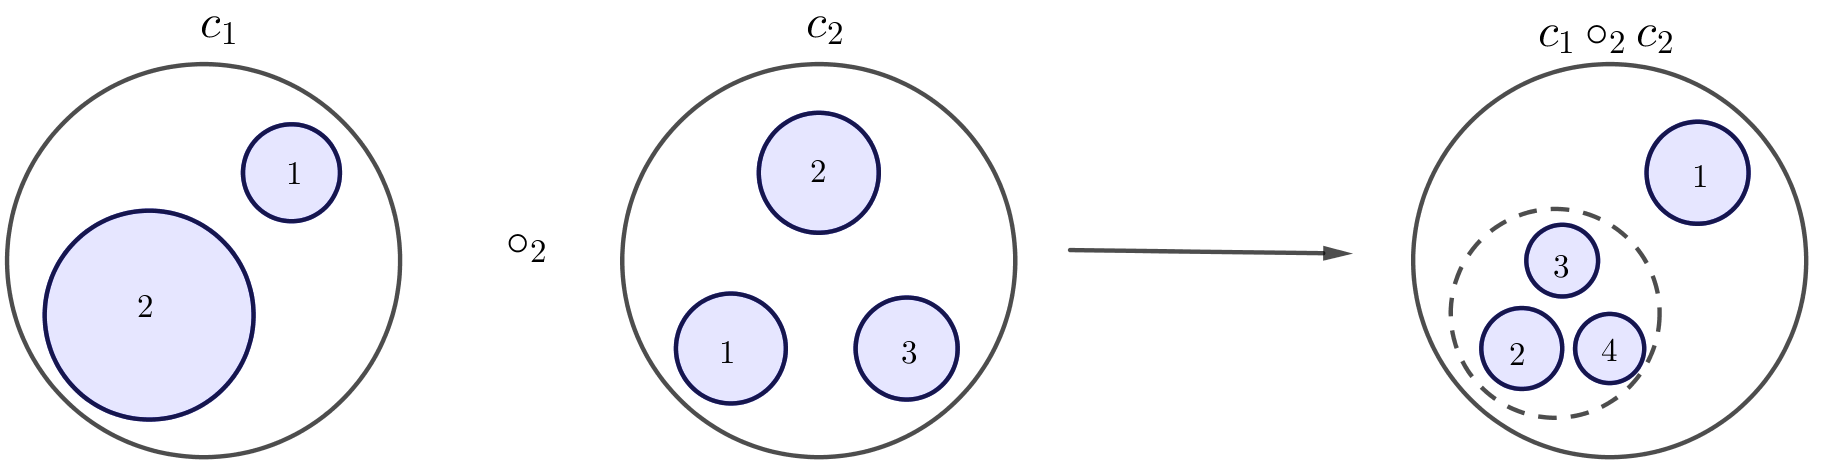
\includegraphics[scale=0.2]{Imagenes/insertion}
	\caption{An insertion $\circ_2:E_2(3)\times E_2(3)\to E_2(5)$.}
\end{figure}
	
\end{frame}

\begin{frame}
	\frametitle{Operad of little disks}
	\begin{figure}
		\begin{tikzpicture}[line cap=round,line join=round,>=triangle 45,x=1.0cm,y=1.0cm]
	\clip(-5.2,-1.5) rectangle (6.92,1.5);
	\draw [line width=2.pt] (0.,0.) circle (1.42cm);
	\draw (-0.2,0.2) node[anchor=north west] {$1$};
	\end{tikzpicture}
	\caption{Identity element $1\in E_2(1)$.}
\end{figure}
\end{frame}
\begin{frame}
	\frametitle{Operad of little disks}
	\begin{figure}[h!]
		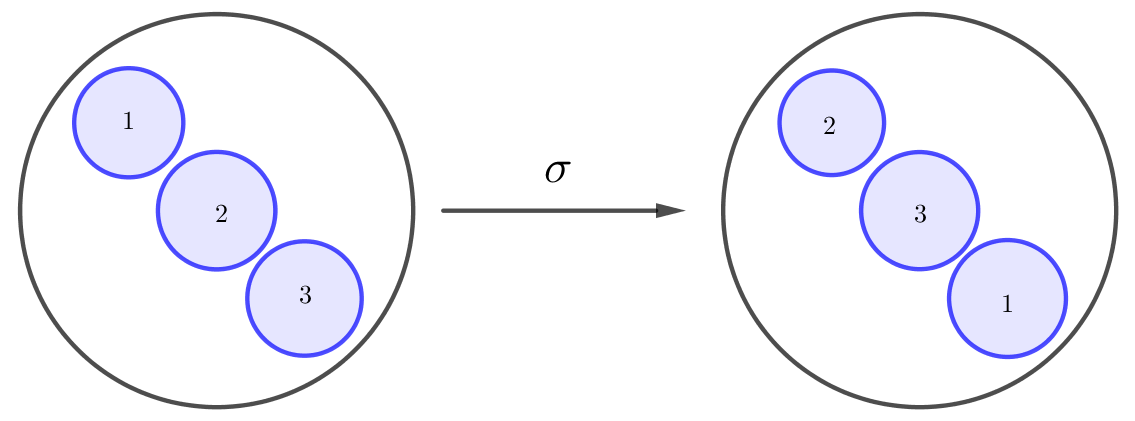
\includegraphics[scale=0.35]{Imagenes//accion}
		\caption{Action of $\sigma=(231)$ on a point of $E_2(3)$.}
	\end{figure}
\end{frame}


\section{Gerstenhaber algebras}

\begin{frame}
	\frametitle{Gerstenhaber algebras}
	\begin{defi}
		Let $k$ be a field of characteristic 0 and $G$ an associative graded $k$-algebra with product $\cdot$. Let $|a|$ denote the degree of an element $a\in G$. Then $G$ is said to be a \textbf{Gerstenhaber algebra} if:
		\begin{itemize}
			\item<2-> The product $\cdot$ is a graded commutative: for every $a,b\in A$ one has $a\cdot b=(-1)^{|a||b|}b\cdot a$
			\item<3-> There is a graded Lie bracked $[,]:G\times G\to G$ such that:
			\begin{itemize}
				\item<4-> $|[a,b]|=|a|+|b|-1$.
				\item<5-> $[b,a]=-(-1)^{(|a|-1)(|b|-1)}[a,b]$ (graded antisymmetry).
				\item<6-> (graded Jacobi identity) $$(-1)^{(|a|-1)(|c|-1)}[[a,b],c]+(-1)^{(|b|-1)(|a|-1)}[[b,c],a]+$$ $$+(-1)^{(|c|-1)(|b|-1)}[[c,a],b]=0$$ 
			\end{itemize}
		\end{itemize}
	\end{defi}
	
\end{frame}




\section{Hochschild cohomology of an associative algebra}
\begin{frame}
	\frametitle{Hochschild complex}
	\begin{defi}
	 We define a \textbf{Hochschild $m$-cochain} $f^m$ of $A$ to be a $k$-module homormorphism $f^m: A^{\otimes m}\to A$. The \textbf{Hochschild complex} is given by the modules $C^m(A;A)=\hom_k(A^{\otimes m}, A)$, where $C^0(A;A)=A$ and the differential
	 \begin{align*}
	 \delta_m f(a_1\otimes\cdots\otimes a_{m+1})&=a_1f(a_2\otimes\cdots\otimes a_{m+1})\\
	  +\sum_{i=1}^m(-1)^if(a_1\otimes\cdots&\otimes a_{i-1}\otimes a_ia_{i+1}\otimes a_{i+1}\otimes\cdots a_{m+1})\\
	 & +(-1)^{m+1}f(a_1\otimes\cdots\otimes a_m)a_{m+1},
	 \end{align*}
	 %extensión lineal de esto
	 \end{defi}
\end{frame}

\begin{frame}
	\frametitle{Hochschild cohomology and cup product}
	\begin{defi}
		The $m$-th \textbf{Hochschild cohomology} of $A$ is defined to be $H^m(A;A)=\ker\delta_m/\im\delta_{m-1}$.
		\end{defi}\pause
	
	\begin{teorema}
		The ring $\{H^*(A,A),\smile\}$ is a graded commutative ring, with grading given by dimension, i.e., if $\eta\in H^m(A,A)$ and $\xi\in H^n(A,A)$, then $\eta\smile \xi =(-1)^{mn}\xi\smile \eta$.
	\end{teorema} 
\end{frame}

%\begin{frame}
%	\frametitle{Cup product}
%	\begin{defi}
%	 For $f\in C^m(A;A)$ and $g\in C^n(A;A)$ define their \textbf{cup product} $f\smile g\in C^{n+m}(A;A)$ by
%	\[
%	f\smile g(a_1\otimes\cdots\otimes a_m\otimes b_1\otimes\cdots\otimes b_n)=f(a_1\otimes\cdots\otimes a_m)g(b_1\otimes\cdots\otimes b_n).
%	\]
%	\end{defi}\pause
%The cup product satisfies the Leibniz rule
%$$\delta (f^m\smile g^n)=\delta f^m\smile g^n+(-1)^m f^m\smile \delta g^n$$\pause
%SI ME QUEDA LARGO QUITAR LAS DEFINICIONES %Con lo cual induce un producto en cohomología
%
%
%\end{frame}

\begin{frame}
	\frametitle{The Hochschild cohomology is a Gerstenhaber algebra}
	
	\begin{teorema}
		Let $A$ be an algebra and $\xi$, $\eta$ and $\zeta$ elements of $H^m(A;A)$, $H^n(A;A)$ and $H^p(A;A)$, respectively. Then there exists a Lie bracket $[,]$ of degree $-1$ such that
		\[
		[\eta, \xi\smile \zeta]=[\eta,\xi]\smile \zeta+(-1)^{m(n-1)}\eta\smile[\xi,\zeta].
		\]
	\end{teorema}\pause
	\begin{teorema}
	The Hochschild cohomology $H^*(A;A)$ is a Gerstenhaber algebra.
\end{teorema} 
\end{frame}
%\begin{frame}
%	\frametitle{Lie Bracket}
%	For $f\in C^m(A;A)$ and $g\in C^n(A;A)$ set
%	\begin{gather*}
%	f\circ_i g(a_0\otimes\cdots\otimes a_{i-1}\otimes b_0\otimes\cdots\otimes b_{n-1}\otimes a_{i+1}\otimes\cdots \otimes a_{m-1})\\
%	=f(a_0\otimes \cdots a_{i-1}\otimes g(b_0\otimes\cdots\otimes b_{n-1})\otimes a_{i+1}\otimes\cdots\otimes a_{m-1})
%	\end{gather*}
%	for $i=0,\dots, m-1$. Note that $f\circ_i g\in C^{n+m-1}(A;A)$.\pause
%	
%	Now set
%	\[
%	f\circ g=\sum_{i=0}^m (-1)^{ni}f\circ_i g.
%	\]
%\end{frame}
%\begin{frame}
%	\frametitle{Lie Bracket}
%	\begin{defi}
%		The bracket is defined by $[f,g]=f\circ g-(-1)^{(n-1)(m-1)}g\circ f$.
%	\end{defi}\pause 
%The bracket also satisfies the corresponding Leibniz rule
%\[\delta[f^m,g^n]=(-1)^{n-1}[\delta f^m,g^n]+[f^m,\delta g^n].\]\pause 
%
%\end{frame}


%\begin{frame}
%	\begin{block}{}
%	\begin{itemize}
%	\item An identity element $1 \in \CC(1)$ such that 
%	$\gamma(1; d) = d$ for $d \in \CC(j)$ and 
%	$\gamma(c; 1,\dots,1) = c$ for
%	$c \in \CC(k)$.
%	
%	\item A right action of the symmetric group $\Sigma_j$ on $\CC(j)$ such that the following equivariance
%	formulas are satisfied for all $c\in \CC(k)$, $d_s \in \CC(j_s)$, $\sigma\in\Sigma_k$, and $\tau_s\in\Sigma_{j_s}$:
%	\[
%	\gamma(c\sigma; d_1, \dots , d_k) = 
%	\gamma(c; d_{\sigma^{-1}(1)}, \dots , d_{\sigma^{-1}(k)})\sigma(j_1, \dots , j_k)
%	\]
%	and 
%	\[
%	\gamma(c; d_1\tau_1, \dots , d_k\tau_k) = \gamma(c; d_1, \dots , d_k)(\tau_1\oplus\cdots\oplus\tau_k),
%	\] 
%	where $\sigma(j_1, \dots , j_k)$ denotes the
%	permutation of $j$ letters which permutes the $k$ blocks of letters determined by the given
%	partition of $j$ (a first block of $j_1$, a second one of $j_2$ letters and so on), and $\tau_1\oplus\cdots\oplus\tau_k$ denotes the image of $(\tau_1, \dots , \tau_k)$ under the evident inclusion of $\Sigma_{j_1} \times \cdots \times \Sigma_{j_k}$ in $\Sigma_j$.
%\end{itemize}
%\end{block}
%
%\end{frame}

\begin{frame}
	\frametitle{Action of the homology operad of litle disks on the Hochschild cohomology}
	
	\begin{teorema}
		Gerstenhaber algebras and $H_*(E_2)$-algebras are the same thing.
	\end{teorema}\pause 
The commutative product is given by 
\[
G^{\otimes 2}\cong k\otimes G^{\otimes 2}\cong H_0(E_2(2))\otimes G^{\otimes 2}\to G
\]
\pause
and the Lie bracket of degree by the
\[
G^{\otimes 2}\cong k\otimes G^{\otimes 2}\cong H_1(E_2(2))\otimes G^{\otimes 2}\to G
\]
	\end{frame}

\begin{frame}
\begin{figure}
	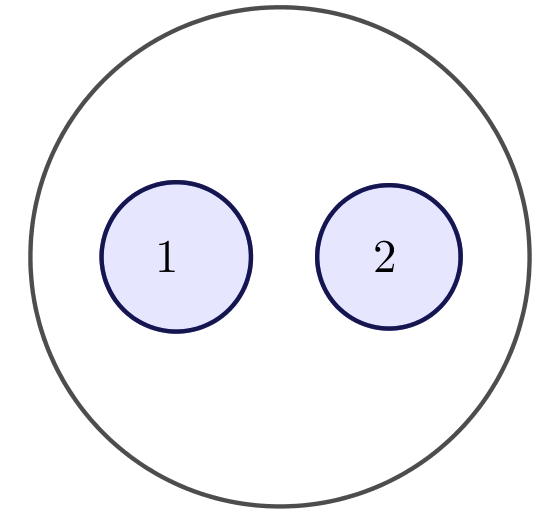
\includegraphics[width=0.3\textwidth]{Imagenes/genera}
	%\hfill
	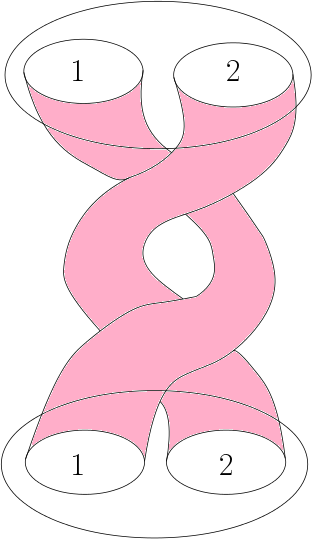
\includegraphics[width=0.3\textwidth]{Imagenes/generador}
	\caption{A generator of $H_0(E_2(2))$ on the left and a generator of $H_1(E_2(2))$ on the right.}
\end{figure}
\end{frame}

\section{Back to the Deligne conjecture}

\begin{frame}
	\frametitle{Back to the Deligne conjecture}
	\begin{block}{The conjecture}
		The action of the homology operad of little disks on the Hochschild cohomology of an associative algebra inducing its Gerstenhaber algebra structure lifts to an action of the chain operad of little disks on the Hochschild complex.
	\end{block}
	\end{frame}

\begin{frame}[fragile]
	\begin{center}
		
	
	\begin{tikzcd}[column sep=60, row sep=30]
	H_*(E_2)\arrow[r,"\text{Gerstenhaber}"] & H^*(A;A)\\
	C_*(E_2)\arrow[u, "q"]\arrow[r, dashed, "?"] & C^*(A;A)\arrow[u, "q"]
	\end{tikzcd}
\end{center}
\end{frame}
\begin{frame}[fragile]
	\begin{center}
		
		
		\begin{tikzcd}[column sep=60, row sep=30]
		H_*(E_2)\arrow[r,"\text{Gerstenhaber}"] & H^*(A;A)\\
		C_*(E_2)\simeq \mathcal{O}?\arrow[u, "q"]\arrow[r, dashed, "?"] & C^*(A;A)\arrow[u, "q"]
		\end{tikzcd}
		%equivalentes en el sentido de que tengan la misma homología
	\end{center}
\end{frame}


\section{Proof of the conjecture}


\begin{frame}
	Cada vez que explique una cosa ponerle un check a lo de antes \url{https://tex.stackexchange.com/questions/132783/how-to-write-checkmark-in-latex} (quizá en operads ponerlo al final al grande y ya)
\end{frame}

\begin{frame}
	Definición de operad y explicación dibujitos (más de los que he hecho en el trabajo)
	
	Operad de endomorfismos y álgebra sobre un operad
	
	Definición de operad en symmetric monoidal categories para que tenga sentido
	
	Comentar gracias al EZ map se hereda la operadición y de ahí a homología
	
	Las operaciones de la homología con los dos dibujitos (en el trabajo solo he metido uno)
	
	Gerstenhaber algebra definición del tirón (en la presentación comentar los criterios de derivación)
	
	Describir el complejo de cadenas sin detallar mucho en que es un complejo de cadenas e ir a su homología con sus propiedades de álgebra de Gerstenhaber (esto ya me relaciona con el último punto)
	
	Recuperar el homology operad y describir la acción sobre un álgebra asociativa
\end{frame}

\begin{frame}
	Retomar la conjetura de Deligne para recordarla y ver que está todo, seguido de un diagrama con las acciones y la que se pregunta si existe poniéndola dashed y con una interrogación de label
	
	Esquema de la prueba (destacar de algún modo las partes en las que me centro)
	
	Pensar qué meto de cada parte
\end{frame}

\end{document}
